%%% PREAMBLE
\documentclass[12pt, a4paper]{article}
%% Packages
% Layout
\usepackage{parskip} % Changes parskip from being indent-based to adding vertical space
\usepackage[margin=2.5cm]{geometry} % Adjust margins to comply with 2,5cm standard
\usepackage{float}
\usepackage{pdflscape}

% Font management (for math and normal text)
\usepackage{sourcesanspro} % Changes font to Source Sans Pro
\usepackage{amssymb, amsmath, amsthm} % Adds math functionality, fonts and environments

% Bibliography and comment management
\usepackage[backend=biber,style=nature]{biblatex} % Bibliography management
\addbibresource{bibliography.bib} % Sets the bibliography-file
\usepackage{csquotes} % Adds babel-biliography compatability
\usepackage{comment} % Comments package for citation-purposes

% Appendix, attachments management
\usepackage[toc,page]{appendix} %
\renewcommand{\appendixtocname}{Appendiks}
\renewcommand{\appendixpagename}{\centering{Appendiks}}
\usepackage{pdfpages} % Including PDF-pages
    \usepackage{eso-pic}
    \usepackage{atbegshi}
    \usepackage{ifthen}
    \usepackage{calc}

% miscellaneous
\usepackage[danish]{translator}
\usepackage[danish]{babel} % Multi-lingual support - danish
\usepackage{lipsum} % Adds lipsum functionality
\usepackage{graphicx} %Titlepage - graphic support
\usepackage[colorlinks = true,linkcolor = blue,urlcolor  = blue,citecolor = blue,anchorcolor = blue]{hyperref} %Titlepage - customizes hyperlinks


%%% Document management
\begin{document}
%% Front matter
    \pagenumbering{roman}
    \begin{titlepage}
    \centering

    \vspace*{1cm}

    % Title and subtitle are enclosed between two rules.
    \rule{\textwidth}{1pt}

    % Title
    \vspace{.7\baselineskip}
    {\huge \textbf{Projekt 1 - Krisen kradser}}

    % Subtitle
    \vspace*{.5cm}
    {\LARGE Efterårssemester 2024}
    
    \rule{\textwidth}{1pt}

    \vspace{1cm}

    % Set this size for the remaining titlepage.
    \large

    % Authors side by side, using two minipages as a trick.

    \begin{table}[h]
        \centering
        \begin{tabular}{cc}
            \begin{minipage}{.5\textwidth}
                \centering
                Jeppe Bøgeskov Bech \\
                {\normalsize \url{jepp9920@zbc.dk}}
            \end{minipage}
            &
            \begin{minipage}{.5\textwidth}
                \centering
                Alexander Schade Knudsen \\
                {\normalsize \url{alex245h@zbc.dk}}
            \end{minipage} 
        \end{tabular}
        
        \vspace{1cm} % Adds vertical space between the rows
    
        \begin{minipage}{.5\textwidth}
            \centering
            Andreas Jensen \\
            {\normalsize \url{andr328q@zbc.dk}}
        \end{minipage}
    \end{table}
    





    

    % More authors can be inserted here with additional minipages.

    \vspace{1cm}

    % Report logo.
    
\includegraphics[width=.7\textwidth]{./assets/zbc_logo_black.jpg}

    \vfill

    % University and date information at the bottom of the titlepage.
    2. x \\
    ZBC Handels- og Teknisk gymnasium Slagelse \\
    Akademisk år 2024-2025 \\
    \today
\end{titlepage}
    \newpage
%    \input{preface/preface.tex}
    \section{Abstract}
This report encompasses the project of developing an application that can be used to manage crises. The application will be developed by a new company called "KEP". 
The application will be developed using a modern application development solution, ensuring optimal performance and compatibility.

\newpage
    \tableofcontents
    \newpage
%% Main body
    \pagenumbering{arabic}
    \section{Forord}
Vi vil gerne rette en tak til Morten Bach Jensen, agronom. Morten hjalp os med vores afgrødeberegner, han hjalp os også med information om sæddosering samt arealallokering, anvendt til beregning.

Vi vil endvidere rette en tak til Jacob Søgaard, Ph.d Video Quality Assessment, som har hjulpet os  \newpage % forord
    \section{Projektstyring}
\subsection{Rollefordeling}
\begin{table}[H]
  \centering
\begin{tabular}{l|l}
           & Roller:                                                \\ \hline
Alexander: & Visionsansvarlig, dokumentarist, strukturering         \\ \hline
Andreas:   & Konceptartist, informationssøgning                     \\ \hline
Jeppe:     & Produktansvarlig, programmør, artistsupervisor, vision
\end{tabular}
\caption{Viser rollefordelingen for vores projekt.}
\end{table}
\subsection{Tidsplan}
Vores tidsplan er håndteret via GitHubs indbygget funktion, se forneden, dog er den opdateret version her:
\begin{figure}[H]
  \centering
  \fbox{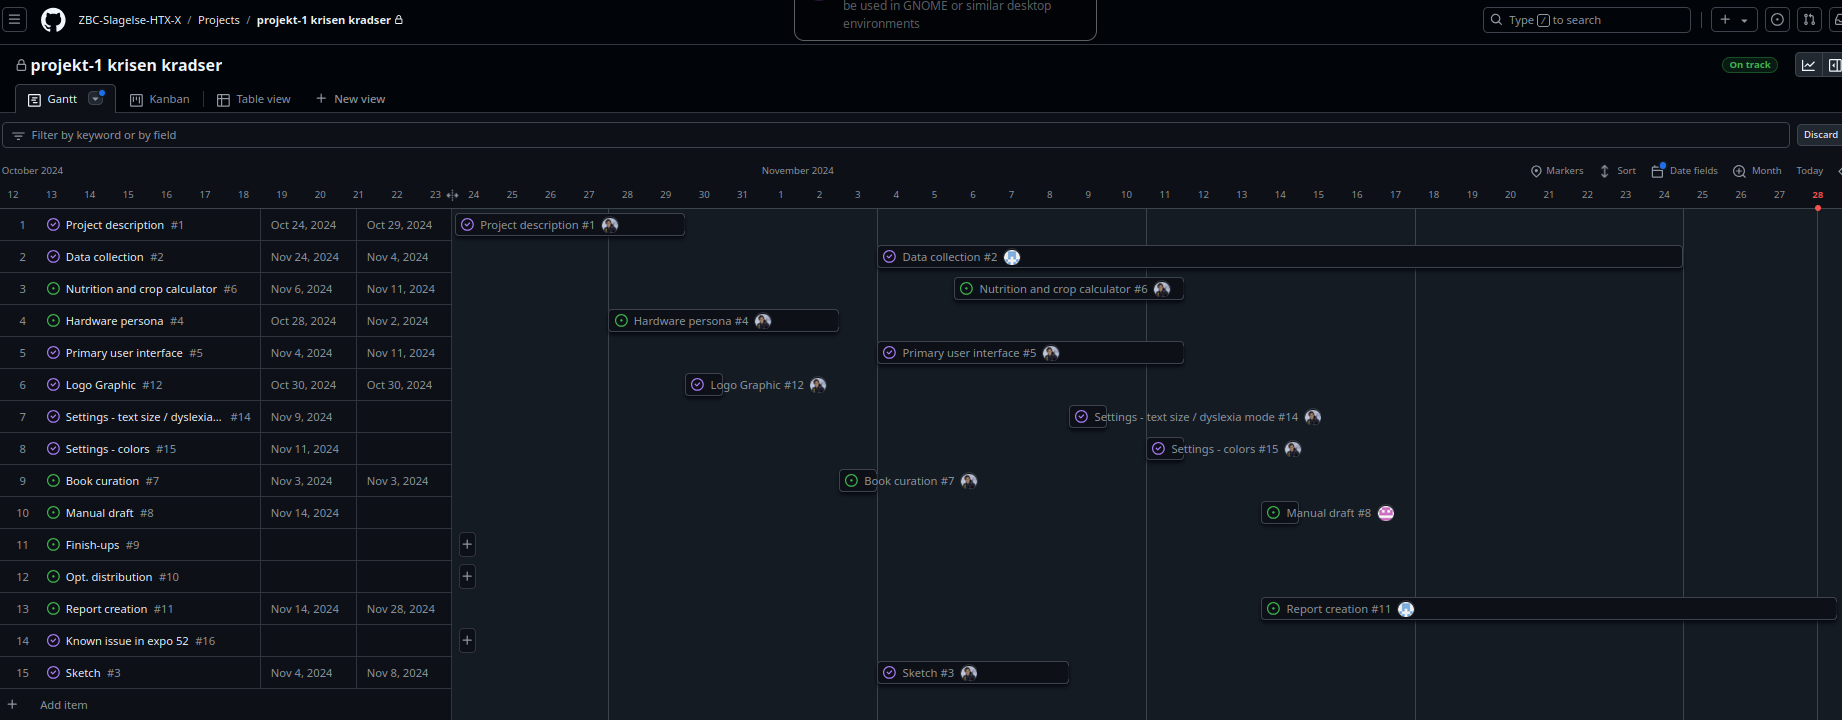
\includegraphics[width=\textwidth]{assets/section_2/2024-11-28_14-25.png}}
\end{figure}

Link til aktuel tidsstyring:
\subsection{Projektmappe}
Link: \href{https://github.com/ZBC-Slagelse-HTX-X/teknologiprojekt-1---Krisen-kradser/tree/main}{Vores GitHub fil}
 \newpage % 
    \section{Problemidentifikation}
\subsection{Idegenerering}
\subsubsection{Mindmap}
Vi har valgt at lave et mindmap, da dette er en effektiv måde at generere ideer på, og få et overblik over hvilke emner der er relevante at beskæftige sig med.
\begin{figure}[H]
    \centering
    \fbox{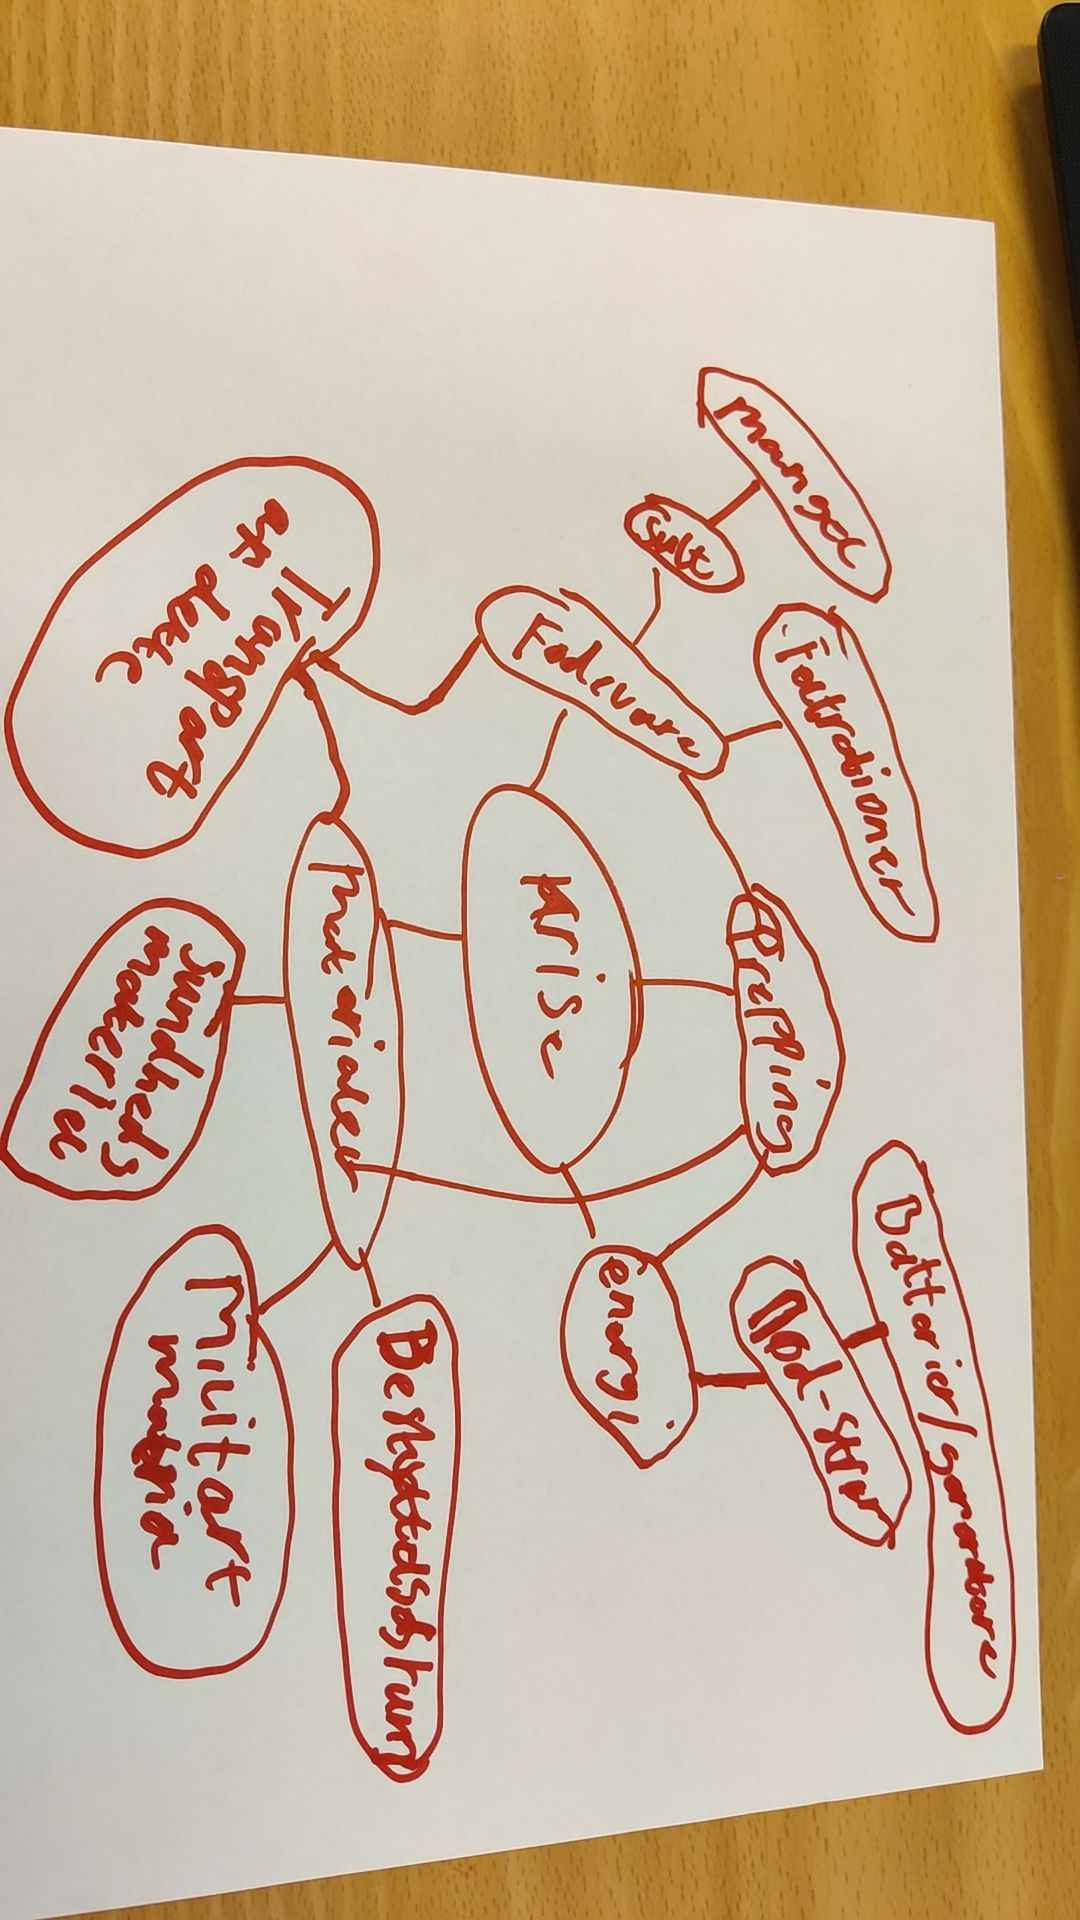
\includegraphics[scale=0.25, angle=90]{assets/section_3/mindmap.jpg}}
    \caption{Viser vores mindmap}
\end{figure}

\subsubsection{Lyskurven}
Lyskurven er en metode, man kan bruge til at sortere ideerne i forhold til hvilke der er mest relevante.
----- Bla bla waffel mere on lyskurvediagrammet -----

\begin{table}[H]
    \centering
    \begin{tabular}{|c|c|c|}
        \hline
        Fødevarer & \textbf{Grøn} \\
        \hline
        Beskyttelsesrum & \textbf{Gul} \\
        \hline
        Nødstrøm & \textbf{Rød} \\
        \hline
    \end{tabular}
    \caption{Viser et meget abstrakt lyskurvediagram i form af en tabel; det vi anvendte}
\end{table}

\subsubsection{Identificering af nøgleproblem}
Ved identifikation af et nøgleproblem, kan man sortere i sine ideer ved at opstille følgende spørgsmål:
\begin{enumerate}
    \item Hvorfor er det her interessant?
    \item Hvem er det interessant for?
    \item Er det noget, vi laver for vores egen fornøjelses skyld?
    \item Er det noget, som en bestemt gruppe i samfundet kan have gavn af, eller er det noget, der er til gavn for alle?
\end{enumerate}
** Spørsmålene som vi her gør brug af er hentet fra systimebogen\footnote{\href{https://projektarbejdet.systime.dk/?id=271}{Projektarbejdet}}

Besvarelsen på disse spørgsmål ser således ud:
\begin{enumerate}
    \item Krisehåndtering er et interessant emne, da det har en stor betydning for alle i samfundet.
    \item Det er relavant for alle.
    \item Nej, ideen med produktet er at kunne hjælpe almindelige mennesker med at håndtere kriser, mindre som store.
    \item Produktet skulle kunne gavne alle, som kunne stå i en krisesituation.
\end{enumerate}

Vi kan nu se, at det mest interessante emne er krisehåndtering, da det har en så stor relavans for grupper i samfundet, og det er noget som vi ser der er behov for. \newpage
    \section{Problemanalyse}
Problemanalysen tager udgangspunkt i nøgleproblemet krisehåndtering jf projektbeskrivelsen, der kan findes som appendiks (\ref{apx:projektbeskrivels}) samt kan man læse kapitlet om problemidentifikation (\ref{sec:problemidentifikation}).

\subsection{Problemtræ}
\begin{figure}[H]
    \centering
    \fbox{\includegraphics[width=\textwidth]{assets/section_3/Problemtræ.jpg}}
    \caption{Viser vores problemtræ}
\end{figure}

\subsection{Kvalitativ metode}
Beredskabstyrelsen har udarbejdet og sendt en opfordring til alle danskere om kriseparathed, hvor de tydeligøre vigtigheden i at være beredt på at kunne håndtere en eventuel krisesituation.
De beskriver i denne, hvordan danskerne skal kunne klare sig selv i 3 døgn, og hvad der skal til for at dette er muligt.
I vores husstande, i det private, er disse opfordringer blevet taget meget seriøst. Men hvad gør man, hvis man løber tør for drikkevand, mad eller lignende? Man kan nødvendivis ikke tilgå hjælp via internettet.
Vi så her en god mulighed, med vores appudviklingsenskaber, at kunne løse dette problem med at lave en app, der kan hjælpe med at håndtere kriser, både forberedene, på kort sigt og på lang sigt.

\subsection{HV-modellen}
Ligedan er HV-modellen blevet brugt for at konkretisere, hvilke trin som tages for at udføre vores projekt.
\paragraph{Hvad?} - Det skal gøres overskueligt og konkret, hvordan man skal handle i en krisesituation.
\paragraph{Hvorfor?} - Det skal gøres, så man kan være beredt i en eventuel krisesituation. Fra et firmasynspunkt er der et stort udbyttepotentiale, da det må forventes, at folk værner om sit og sine næstes liv. Desuden er det sandsynligt, at eftersom beredskabstyrelsen har varslet information om kriseparathed \cite{krisemanual}, at man via en aftale med staten eventuelt kunne få et subsidium til udarbejdelsen af en sådan applikation, som heri benævnes.
\paragraph{Hvem?} - Projektet skal udarbejdes af en nyopstartet virksomhed, her fiktivt, "KEP". Se mere om "KEP"-størrelsen under kapitlet om distribution og praksisudførelse \ref{sec:distribution}.
\paragraph{Hvordan?} - Det skal gøres ved at lave et program, der gør overstående jf. "hvad?", via en moderne applikationsbyggeløsning, således at denne finde den gyldne vej imellem optimisering og kompatabilitet.

 \newpage
    \section{Produktprincip}
\subsection{Målgruppe}
Det tilsigtes, at produktet skal være tilgængeligt for alle danskere, da kriser ikke diskriminerer. Det betyder i praksis, at personer, der har diverse handicap, skal være i stand til at kunne produktet, herunder folk, som er ord- eller farveblinde.
\subsection{Kravspecifikation}
Da det må forventes, at produktet skal kunne anvnedes i tilfælde af et nedbrud af internettet, herfor skal produktet kunne fungere uden internetforbindelse dvs. applikationen skal være offline--og da det er planen, at appen skal indeholde videoer, skal disse ligedan nedhentes.
Desuden skal produktet være simpelt og intuitivt at forstå, herunder have ordforklaringer og selve brugergrænsefladen skal være let at navigere rund i og følge nuværende UI-standarder.
Produktet skal ligedan være et kompromis mellem design og letvægtighed, herved forstås der, at appen ikke er resursekrævende, således at selv ældre hardware kan tilgå appen.

Hermed på listeform:
\begin{itemize}
    \item Offlinefunktionalitet
    \item Letvægtighed
    \item Simpel brugergrænseflade samt ordforklaringer
\end{itemize}

\subsection{Konkurrenter}
Der er ikke umiddelbart nogen decideret konkurrent til produktet, især ikke på det danske marked, som henvendes til, men der et utal af videoer og guides om overlevelse i det vilde og diverse beregnere på internettet, men her adskiller det forslået produkt sig ved at være tilgængeligt uagtet internetforbindelse, mere omfattende og tilgængeligt på dansk. \newpage
    \section{Produktudformning}
\subsection{Overordnet}
Koden er opbygget, således at den kan skrives som en pseudo-webapplikation, sidenhen anvendes en "bro", der gør til en native applikation og kompatibel med de mest almindelige styresystemer, herunder IOS (Apples mobile styresystem) og Android\footnote{Selvsamme teknik anvendes af højtprofilerede virksomheder, såsom Facebook, Discord og Tesla. Læs mere her: \href{https://reactnative.dev/}{reactnative.dev}}.

\subsection{Kodestack}
\subsubsection{Framework - React Native}
React Native er et framework\footnote{Et framework er en samling af biblioteker, der gør det lettere at skrive kode på en standardiseret måde, hvori en masse valg er taget på forhånd}, der muliggør udvikling af native\footnote{Native betyder at applikationen kører direkte på enheden} applikationer til IOS og Android. 
\subsubsection{Sub-Framework - Expo}
Expo er et framework, der er bygget omkring React Native, der muliggør at køre en pågældende React Native-applikation igennem deres egen platform, Expo Go, hvorfor man ikke behøver at kompile koden, dvs. oversætte programmeringskoden til eksekverbar maskinekode, efter hver ændring, såfremt man vil teste den på en fysisk enhed. 
\subsubsection{Runtime - Node.js}
Node.js er den runtime, der muliggør at applikationen kan køre på en enhed fremfor i en browser, da programmeringssproget JavaScript oprindeligt var designet til at køre udelukkende i et browser-miljø. 
\subsubsection{Database - MongoDB*}
Ideen var oprindeligt at have en meget let applikation, der kunne nedhentes fra et styresystems nativ app-bibliotek, hvorefter denne ville prompte brugeren til at nedhente ekstrapakker, fx videoer og manualer, fra vores egen server, som skulle være administreret via MongoDB. MongoDB er en program, som tillader en at lave og administrere enNoSQL-database, hvilket er en mere fleksibel database end traditionelle SQL-databaser. 
\subsubsection{Programmeringsprog - Typescript}
Typescript er et programmeringssprog udviklet af Microsoft, som bygger på JavaScript. Typescipt bruger stærke datatyper, hvilket vil sige, at datatypen angives per data. Typescript anvendes i denne applikation, fordi det er et kompilersprog, hvilket vil sige, at fejl kan blive fanget, når koden kompileres, fremfor i runtime, mens programmet kører, hvilket er en stor fordel i programmeringsprocessen, da det hindrer, at der kommer oversete fejl i koden.
\subsection{Brugergrænseflade}
Brugergrænsefladen er det, brugeren oplever, når han interagerer med applikationen. Brugergrænsefladen er blevet tegnet i Figma, et program, som er speciallavet til at konstruere brugergrænseflader, bl.a. har den prælavede elementer, fx knapper og tekstinputfelter, desuden kan dette gøres interaktivt. 
\subsubsection{Konceptdesign}
Jf. appendiks INSERT FIGURE er følgende skitser blevet udarbejdet. Herefter er disse blevet implementeret i selve applikationen. Brugergrænseflade består primært af en bjælke, der er placeret i bunden af skærmen, hvorfra brugeren kan navigere mellem forskellige sider.
\subsubsection{Design}
\subsection{Kodegennemgang}
 \newpage
    \newpage
%% Back matter
     \printbibliography[heading=bibintoc,title={Litteraturliste}]
     \begin{appendices} \newpage
         \section{Projektbeskrivelse \label{apx:projektbeskrivels}} \newpage
        \renewcommand*{\thepage}{A\arabic{page}}
        
\includepdf[pages=-,delta=5 5,frame=true,landscape=true,nup=1x2,pagecommand={\thispagestyle{plain}}]{./project description/project_description.pdf}
        \section{Konceptart} \label{apx:konceptart} \newpage
        \renewcommand*{\thepage}{B\arabic{page}}
        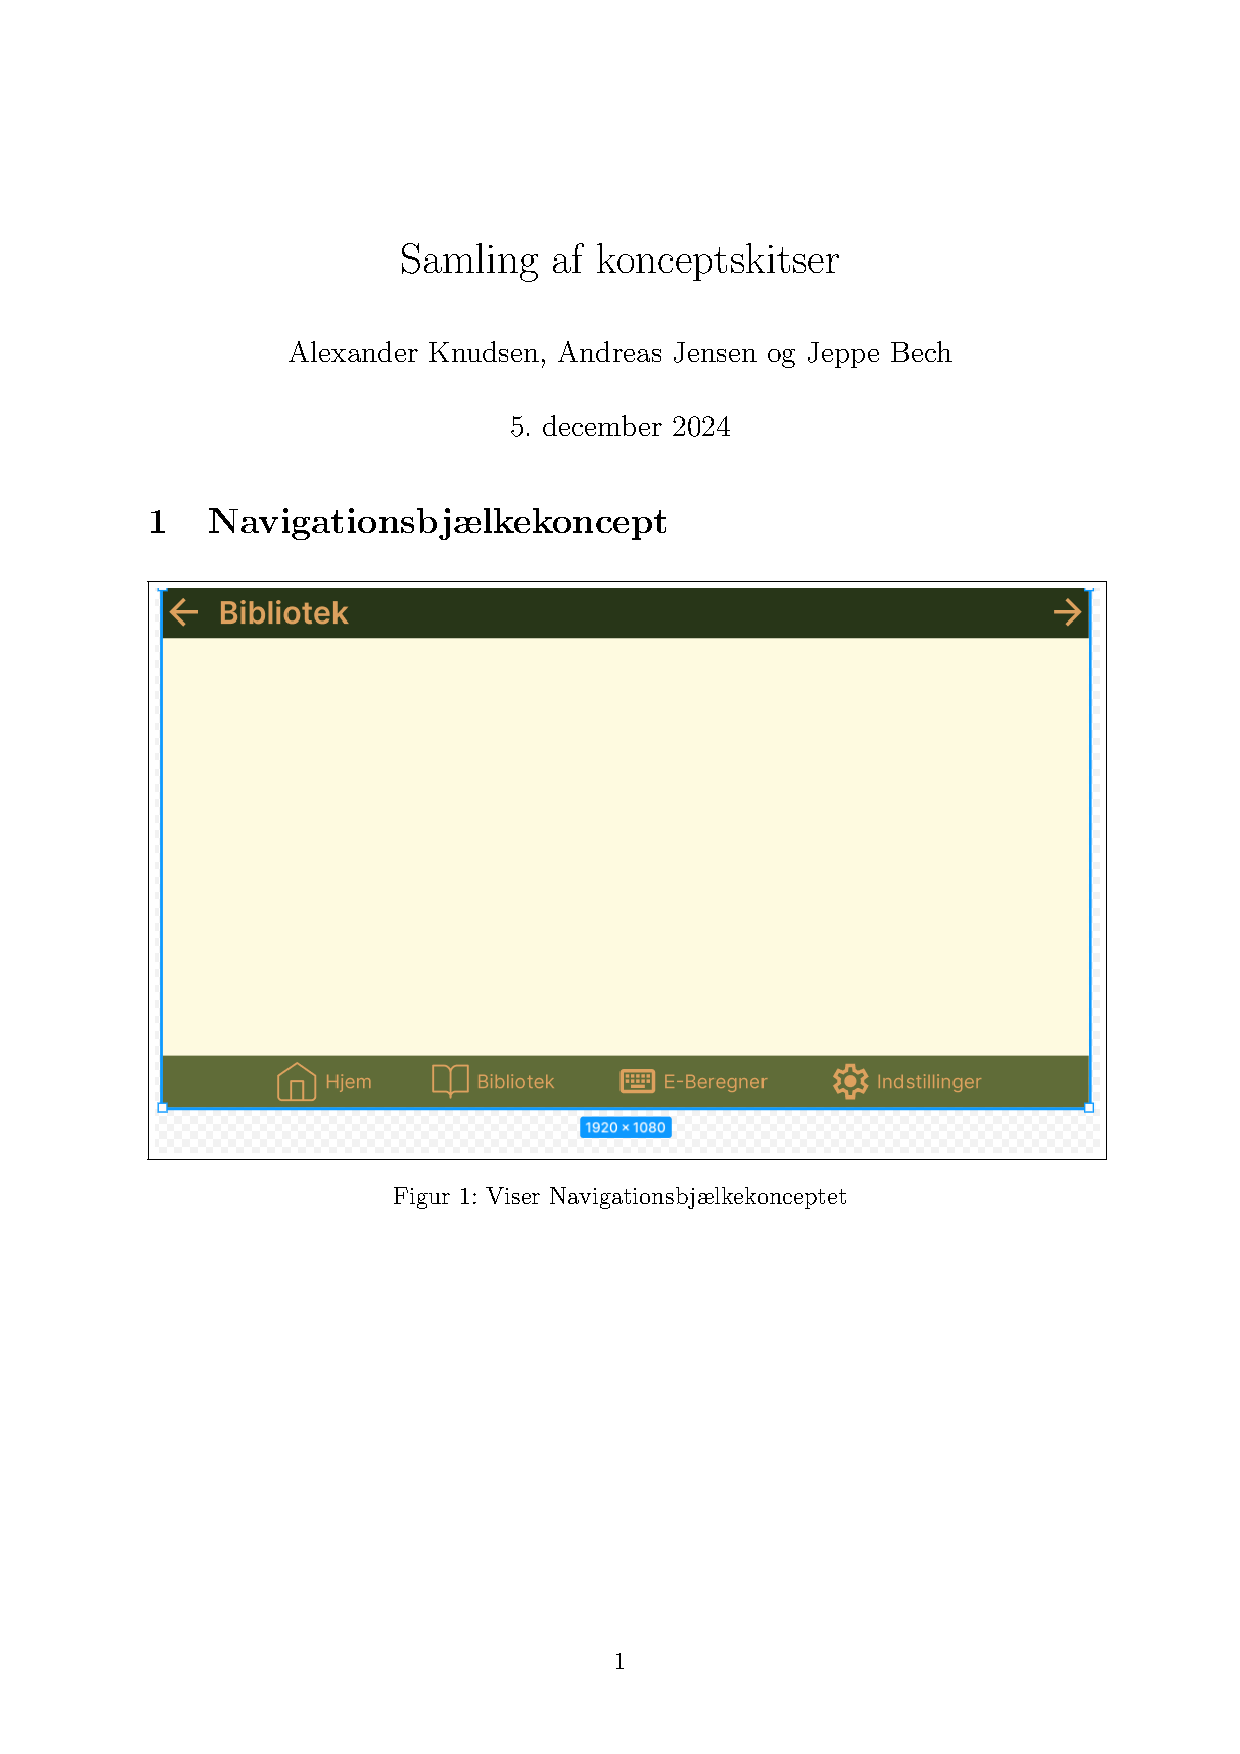
\includepdf[pages=-,delta=5 5,frame=true,landscape=true,nup=1x2,pagecommand={\thispagestyle{plain}}]{./concept_art/concept_art.pdf}
        % \renewcommand*{\thepage}{B\arabic{page}}
%         \includepdf[pages=-,delta=5 5,frame=true,landscape=true,nup=1x2,pagecommand={\thispagestyle{plain}}]{Log/log.pdf}
%         \renewcommand*{\thepage}{\arabic{page}}
     \end{appendices}
  \end{document}
